%!TEX root = ../sample-acmlarge.tex
Although the IREOS index was the first, and so far the only, internal index devoted to bridging the gap related to the internal evaluation of outlier detection results \cite{zimek2013,marques2015}, it has the main limitation of restricting to directly evaluate only top-$n$ (binary) outlier detection results $\mathbf{S}$. Without previously know the number of outliers in the dataset $n$, it is not possible to evaluate a solution given as outlier scoring $\mathbf{y}$. In this section, we devise means to extend IREOS to evaluate a collection of candidate solutions $\mathbf{y}$ in the absence of labels and independent of a choice of $n$.

\subsection{Internal Evaluation of Top-n Outlier Detection Results}
Since the observations $\mathbf{x}_i$ are sorted and ranked according to their degree of outlierness $y_i$ and the threshold in the ranking is established, the top-$n$ observations can be labeled as outliers. Even though it is clear that the best solution must rank all outliers before all inliers and the worst solution must rank all inliers before all outliers, there are $n!$ different possible best top-$n$ solutions equally well rated. However, the truly best outlier solution should rank more obvious or clear outliers before less obvious outliers before those that could be outliers or inliers and so on. This issue was already discussed and addressed by \cite{schubert2012} in the context of the external evaluation of outlier detection, once that the main external measures (\textit{e.g.} ROC AUC and $prec@n$) cannot make such distinction. As well as these external measures, IREOS cannot differentiate the quality of these $n!$ different possible best solutions.

We start the IREOS extension addressing the problem discussed above, in order to make possible distinguish the quality of the ranks among the top-$n$ observations, we introduced weights in the Equation \ref{eq:ireos:avg_curve} where the average curve of separability is defined, so that the average curve of separability becomes a weighted average curve of separability,
%\begin{equation}
%\int_{\gamma = 0}^{\gamma_{max}} \bar{p}(\gamma) = \int_{\gamma = 0}^{\gamma_{max}} \frac{1}{\sum_{\mathbf{x}_i \in \mathbf{S}} w_i} \sum_{\mathbf{x}_i \in \mathbf{S}} p(\mathbf{x}_i, \gamma) w_i
%\label{eq:w_avg_sep}
%\end{equation}
\begin{equation}
\int_{\gamma = 0}^{\gamma_{max}} \bar{p}(\gamma) = \int_{\gamma = 0}^{\gamma_{max}} \sum_{\mathbf{x}_i \in \mathbf{S}} p(\mathbf{x}_i, \gamma) w_i, \sum_i w_i = 1
\label{eq:w_avg_sep}
\end{equation}
where $w_i$ stands for the weight associated with the observation $\mathbf{x}_i$. The use of weights in the outlier evaluation was already discussed by \cite{schubert2012}, the authors argue that the choice of a score-based approach is a good option for several reasons, but when comparing different methods that have different scales, some kind of normalization is unavoidable. Following the authors' recommendation, we use the outlier scoring normalization framework proposed by \cite{kriegel2011}, as this framework proposes a variety of normalization methods based on statistics and distribution fitting that can accommodate several outlier detection algorithms. Thus, the normalized outlier scores $w_i$ are used as the weights associated to observations $\mathbf{x}_i$.

By introducing the score-based weights we expected that in the truly best solution, the outlier scores and the separabilities of the more obvious outliers to be higher, whereas in a false best solution, while the outlier scores of the less obvious outliers are expected to be higher, their separabilities are expected to be lower. Therefore, when combined the higher outlier scores with the higher separabilities and the lower outlier scores with lower separabilities of the truly best solution, it will produce a larger AUC, when compared with AUC produced by a false best solution that combines higher outlier scores with lower separabilities and lower outlier scores with higher separabilities. An illustrative example is provided in Fig. \ref{fig:ilustration}. In Fig. \ref{fig:data} three observations are labeled as outliers in a hypothetical top-$n$ outlier detection solution, a more obvious outlier (blue square), a less obvious outlier (green circle) and a not obvious outlier (red diamond). Their separabilities are individually assessed in the Fig. \ref{fig:ind_avg_curv}. In Fig. \ref{fig:avg_sep_curv} two variations of this top-$n$ outlier solution are presented, differing in the outlier scores ranking. The named truly best solution ranks the more obvious outlier (outlier score 1) before the less obvious outlier (outlier score 0.75) before the not obvious outlier (0.51), the reverse ranking of the false best solution that ranks the not obvious outlier (outlier score 1) before the less obvious outlier (outlier score 0.75) before the more obvious outlier (0.51). These two different solutions would be equally well rated for the main external measures AUC ROC and $prec@n$ as well as IREOS before the proposed extension. However, using the proposed weighted average curve of separability the index can properly evaluate the solution, as expected the truly best solution has a larger AUC than the false best solution, so the quality of the truly best solution is higher than the false best solution.

\begin{figure}[h!]
\center
\subfloat[Illustrative dataset]{\label{fig:data} 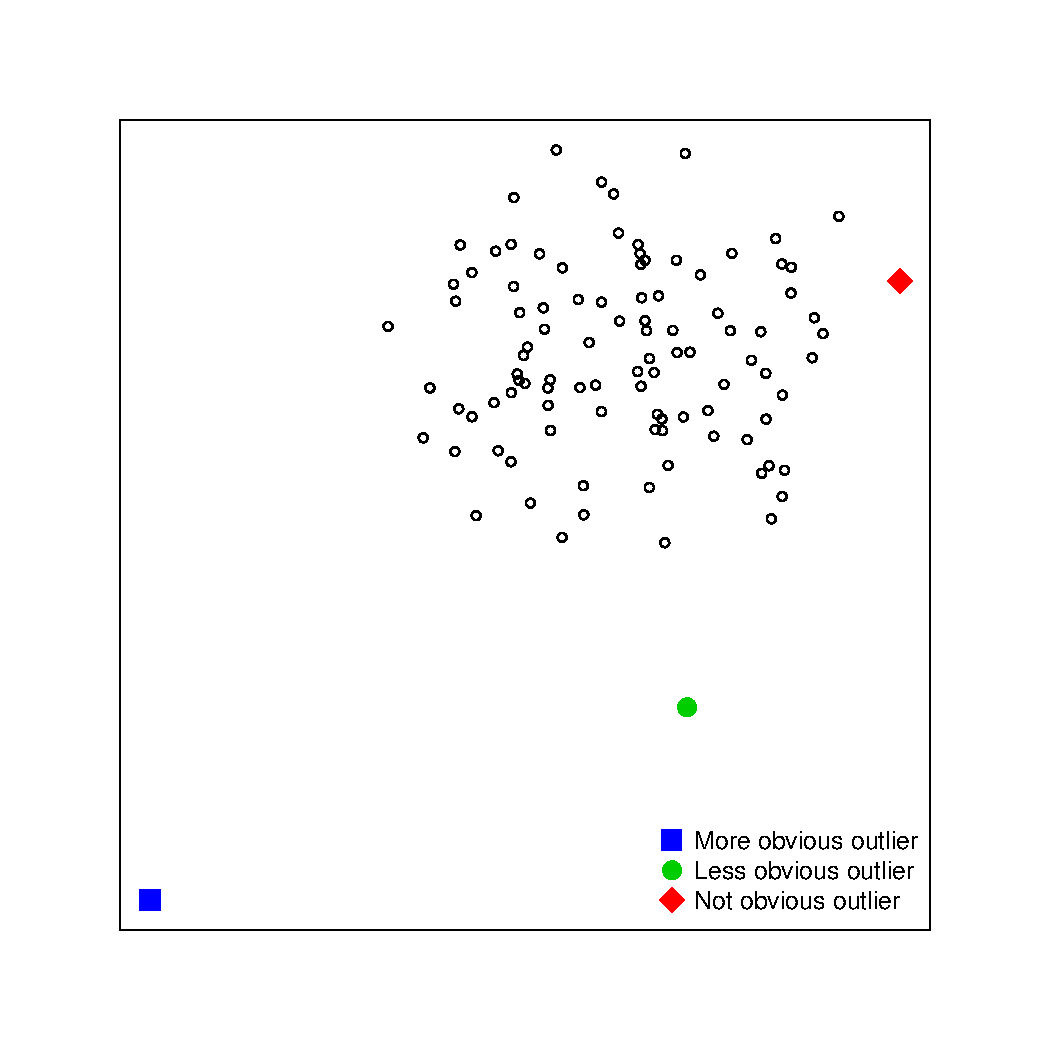
\includegraphics[width=4.7cm]{figs/data.pdf}}
\qquad
\subfloat[Individual separability curves]{\label{fig:ind_avg_curv} 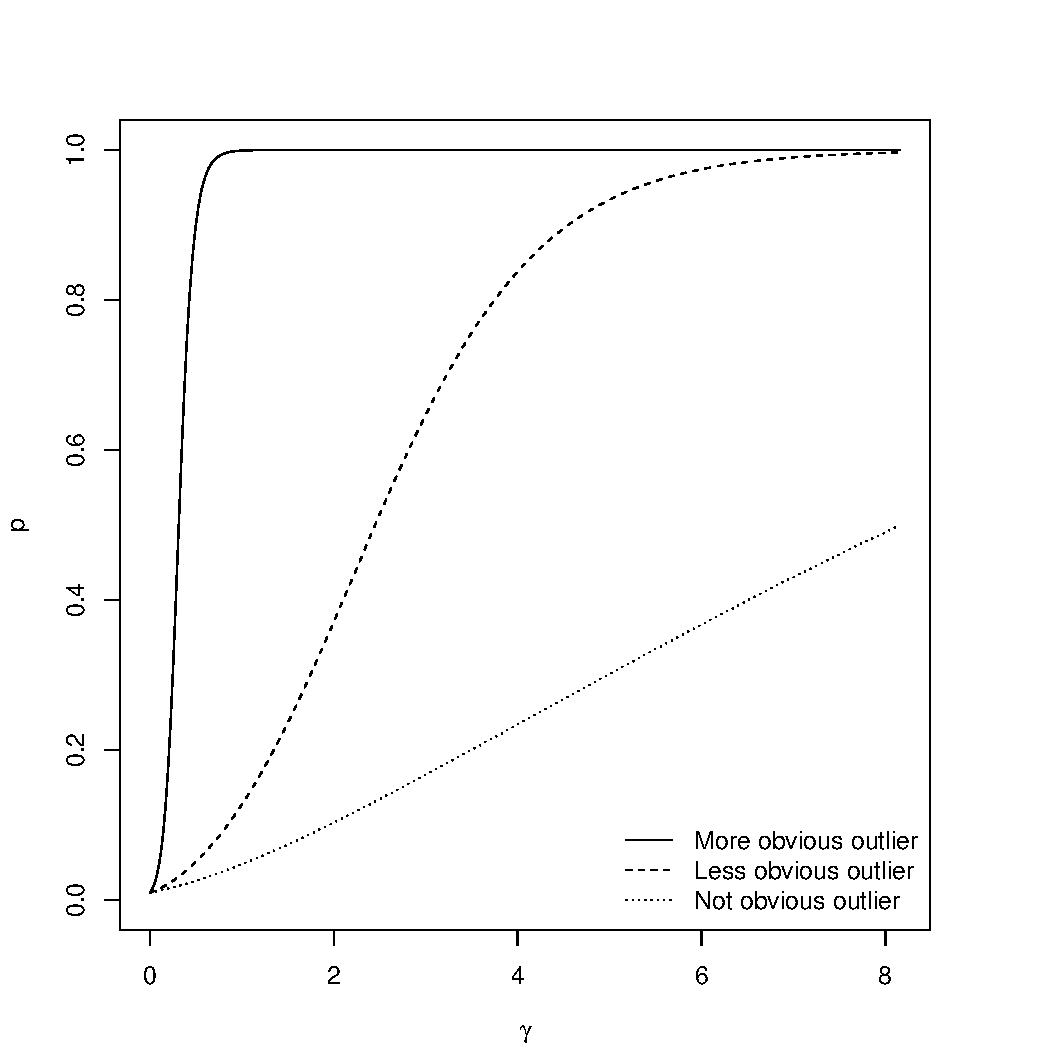
\includegraphics[width=4.7cm]{figs/sep_curves.pdf}}
\qquad
\subfloat[Weighted average curve of separability]{\label{fig:avg_sep_curv} 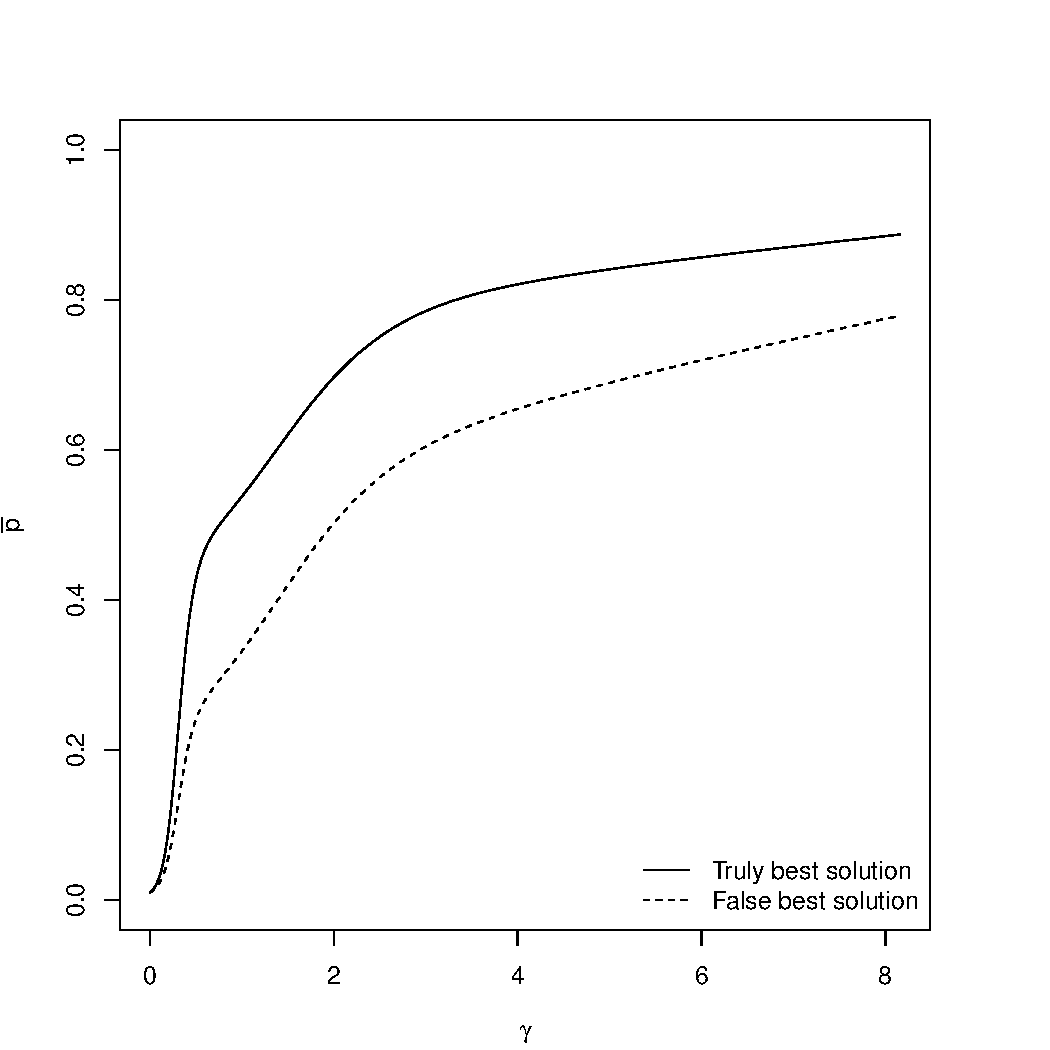
\includegraphics[width=4.7cm]{figs/avg_sep_curves.pdf}}
\caption{Illustrative example of a top-$n$ outlier solution: In \ref{fig:data} the top three observations are labeled as outliers; Their separabilities are individually assessed in \ref{fig:ind_avg_curv}; The outlier scorings of the two different top-$n$ solutions are evaluated in \ref{fig:avg_sep_curv}, the outlier scores of the more obvious outlier, the less obvious outlier and not obvious outliers are respectively 1, 0.75, 0.51 for the truly best solution and 0.51, 0.75, 1 for the false best solution}
\label{fig:ilustration}
\end{figure}

The extension proposed here is computed similarly to the original index presented in the Equation \ref{eq:original_ireos}. However, instead of use the average curve of separability (Equation \ref{eq:ireos:avg_curve}) we use the weighted average curve of separability (Equation \ref{eq:w_avg_sep}):
%\begin{equation}
%I(\mathbf{S}) = \frac{1}{n_{\gamma}} \sum_{l = 1}^{n_{\gamma}} \left( \frac{1}{\sum_{\mathbf{x}_i \in \mathbf{S}} w_i} \sum_{\mathbf{x}_i \in \mathbf{S}} p(\mathbf{x}_i, \gamma_l) w_i \right)
%\label{eq:ext_ireos}
%\end{equation}

\begin{equation}
I(\mathbf{S}) = \frac{1}{n_{\gamma}} \sum_{l = 1}^{n_{\gamma}}  \sum_{\mathbf{x}_i \in \mathbf{S}} p(\mathbf{x}_i, \gamma_l) w_i, \sum_i w_i = 1
\label{eq:ext_ireos}
\end{equation}

Note that giving the same scores for all observations labeled as outliers the index of the Equation \ref{eq:ext_ireos} will be reduced to the original index of the Equation \ref{eq:original_ireos}, where the followed assumption is that all the observations labeled are equally outliers.

\subsection{Internal Evaluation of Scoring Outlier Detection Results}
From the first extension is easy to note that such index could be trivially extended in order to evaluate the whole outlier scorings. As we intend to evaluate the solution without make the assumption that the number of outliers in the dataset is known, we take into account the whole dataset $\mathbf{X}$ in the evaluation, instead of the only top-$n$ outlier observations present in $\mathbf{S}$:
%\begin{equation}
%I(\mathbf{S}) = \frac{1}{n_{\gamma}} \sum_{l = 1}^{n_{\gamma}} \left( \frac{1}{\sum_{\mathbf{x}_i \in \mathbf{X}} w_i} \sum_{\mathbf{x}_i \in \mathbf{X}} p(\mathbf{x}_i, \gamma_l) w_i \right)
%\end{equation}

\begin{equation}
I(\mathbf{S}) = \frac{1}{n_{\gamma}} \sum_{l = 1}^{n_{\gamma}} \sum_{\mathbf{x}_i \in \mathbf{X}} p(\mathbf{x}_i, \gamma_l) w_i, \sum_i w_i = 1
\label{eq:compl_ext_ireos}
\end{equation}

As outlier detection is a rather imbalanced problem, where only the top observations are important, the index will give more importance to observations with high scores, whereas the inliers scores that dominate the problem will be almost irrelevant, once they usually do not vary much at all and will tend to 0 with the scoring normalization. This important property makes the quality of the solution do not be influenced by the inliers, even though they are the majority, and slightly penalize the exchange between observations with similar scores (\textit{e. g.} the exchange between clear inliers, or between clear outliers), while the exchange between observations with high contrast in the outlier scorings has a higher penalization (\textit{e. g.} the exchange between a clear outlier and a clear inlier).

\subsubsection{Modeling clumps}
The possible presence of clumps in the data set induces IREOS to provide the users with an optional control mechanism to adjust their expectations about clump sizes. The maximum clump size ($m_{cl}$) is responsible for determining the fraction of the cost $C$ associated with soft margin classifier that the observations labeled as outliers will receive, this fraction of the penalty ($\beta$) determine how much these observations will individually affect the separabilities from each other. Originally, the observations labeled as inliers receive the full cost $C$, and the observations labeled as outliers receive only a fraction $\beta$ of this full cost. Being $\beta = \frac{1}{m_{cl}}$, so that, one needs $m_{cl}$ observations (a full clump) labeled as outliers to get the same impact as a single inlier. However, here it does not exist anymore the inliers and outliers labeling, instead, the degree of outlierness takes place. In order to extend IREOS to continue supporting the modeling clumps, the penalty cost associated with observations $\mathbf{x}_i$ ($C(\mathbf{x}_i)$) will be given according to their degree of outlierness:
%\begin{equation}
%C(\mathbf{x}_i) = C \times \left( \frac{1}{m_{cl}} \right)^{\left(1-\frac{rank(\mathbf{x}_i)}{N - 1}\right)}
%\end{equation}

\begin{equation}
C(\mathbf{x}_i) = C \cdot \beta^{w_i}
\end{equation}
where $\beta$ continue as $\beta = \frac{1}{m_{cl}}$ and ${w_i}$ is the normalized outlier score associated with the observation $\mathbf{x}_i$. 

Note that the modeling clumps is reduced to the one used before when all the inliers receive 0 as outlier scorings ($\beta^0 = 1$, full cost for inliers) and all the outliers receive 1 as the outlier scorings ($\beta^1 = \frac{1}{m_{cl}}$, $\frac{1}{m_{cl}}$ of the cost for outliers).

%Note that the index will be reduced again to the original index when all the inliers receive 0 as outlier scorings and all the outliers receive 1 as the outlier scorings.

<<<<<<< HEAD
\subsubsection{Adjustment for Chance}
The extension as described above is ready to be used in practice if one is only interested in comparing in relative terms a set of different candidate solutions, \textit{e.g.} for model selection. However, the interpretation of the index for individual solutions, \textit{e.g.} for statistical validation, can be very misleading. As well as IREOS, its extension also provides a certain positive value even when evaluating purely random solutions. To make things worse, such a value is data dependent. In fact, note from Figure \ref{fig:ilustration} that even inliers will exhibit a non null value for the AUC of separability. In order to avoid this misleading, the IREOS index was adjusted for chance using the classic statistical framework for chance adjustment \cite{hubert1985}. Here, we will follow the same classic statistical framework,

\begin{equation}
I_{adj}(S) = \frac{I(S) - E\{I\}}{I_{max} - E\{I\}}
\end{equation}
where $I_{adj}(S)$ is the resulting (adjusted) index, $I(S)$ is the original index (Equation \ref{eq:ext_ireos}), $I_{max} = 1$ is the maximum value that the index can take, and $E\{I\}$ is its expected value assuming that the outlier scorings of a solution are randomly assigned. For random solutions, $I_{adj}$ is expected to take values around zero. The maximum is still 1, but the index now can take negative values to indicate solutions even worse than what one would expect to obtain by chance.

Assuming that the scorings were randomly generated, there are two terms in Equation \ref{eq:ext_ireos} that are affected: 1) Directly, the weights $w_i$'s that are obtained from the scorings normalization; and 2) indirectly, the separability values $p(\textit{x}_i)$'s that can assume infinite values of separability depending on the scorings of the other observations and the value of $m_{cl}$ used.

\begin{equation}
E\{I\} =  \frac{1}{n_{\gamma}} \sum_{l=1}^{n_{\gamma}} E\{ \bar{p}(\gamma_l) \}
\end{equation}

\begin{equation}
E\{ \bar{p}(\gamma_l) \} = E\{ p(\mathbf{x}_i, \gamma_l) \}
\end{equation}


\subsection{Approximate Computation}
We are aware of the high computational complexity needed to evaluate the candidate solutions $\mathbf{y}$. For each candidate solution $\mathbf{y}$, we need to training $N \cdot n_{\gamma}$ classifiers. The maximum margin classifiers are known for the high asymptotic computational complexity $\mathcal{O}(N^3)$\footnote{SVM due to the support vector ($sv$) properties is $\mathcal{O}(sv \cdot N^2)$, but the worst case where $sv = N$ it becomes $\mathcal{O}(N^3)$ again}. Thus, the overall complexity to evaluate a candidate solution $\mathbf{y}$ is, in general, $\mathcal{O}(n_{\gamma} \cdot N^4)$. In order to make the computation of the index treatable for large datasets, we provide approaches to avoid unnecessary computations on the three parts responsible to the complexity of the index: Separability curves ($n_{\gamma}$),  Observations' separability ($N$) and Classifiers ($N^3$).

\subsection{Separability curves}
In practice to calculate the separability curves, and consequently the index, we need to discretize the $\gamma$ values into $n_{\gamma}$ values in the interval $[0, \gamma_{max}]$, so that the classifiers can be trained to calculate the $\bar{p}(\gamma)$ for each $\gamma$. In the experiments performed on \cite{marques2015}, this interval was discretized in  $n_{\gamma} = 100$ values. Although this value is empirically sufficient for a good approximation of the area of the separability curve, it is not possible to have an idea of how the associated error behaves as the value of $n_{\gamma}$ varies, so that the user can choose how much he wants to lose in accuracy to gain in performance. In addition, an approach that discretizes values equally (or even logarithmically) may not be the most efficient, since $\gamma$ values can be attributed in less critical regions of the curve, \textit{e.g.}, when the curve has already become flat and there would be no need for more values in that region.

For a more efficient calculation of the index, instead of using a fixed number $n_{\gamma}$, we will use a variable number $n_{\gamma}$ according to some user-specified tolerance of an estimated error of the index. In order to do that, we will apply the technique of adaptive quadrature, or adaptive numerical integration \cite{kuncir1962,gonnet2012,burden2016}. This technique will approximate the separability curve area by subdividing it recursively and adaptively into smaller subintervals until each subinterval reaches the user-specified precision. This procedure is illustrated in the Figure \ref{fig:approx_trap}, where the three curves presented in the Figure \ref{fig:ind_avg_curv} are approximated by this procedure. Initially in Figure \ref{fig:approx_3p}, the separability curve represented by the solid line is approximated by the dashed line with only three points. Since the approximation is not good enough, the separability curve is divided into two parts and the area of these two parts are calculated independently (Figure \ref{fig:approx_5p}, the division of the separability curve is marked by the dotted line). Since the area of the right division has already reached a good approximation, only the left part will be further subdivided (Figure \ref{fig:approx_7p}). This procedure is repeated recursively, until each subdivision reaches a sufficiently good approximation (Figure \ref{fig:approx_21p}). The other two separability curves of Figure \ref{fig:ind_avg_curv} are approximated by the same procedure in Figures \ref{fig:approx_3pcv2}-\ref{fig:approx_9p} and \ref{fig:approx_3pcv3}. Note that the number of points needed to achieve a good approximation varies in each case, and in general, the smaller the separability of the observation, the fewer points are needed to approximate its separability curve.

\begin{figure}[h!]
\center
\subfloat[]{\label{fig:approx_3p} 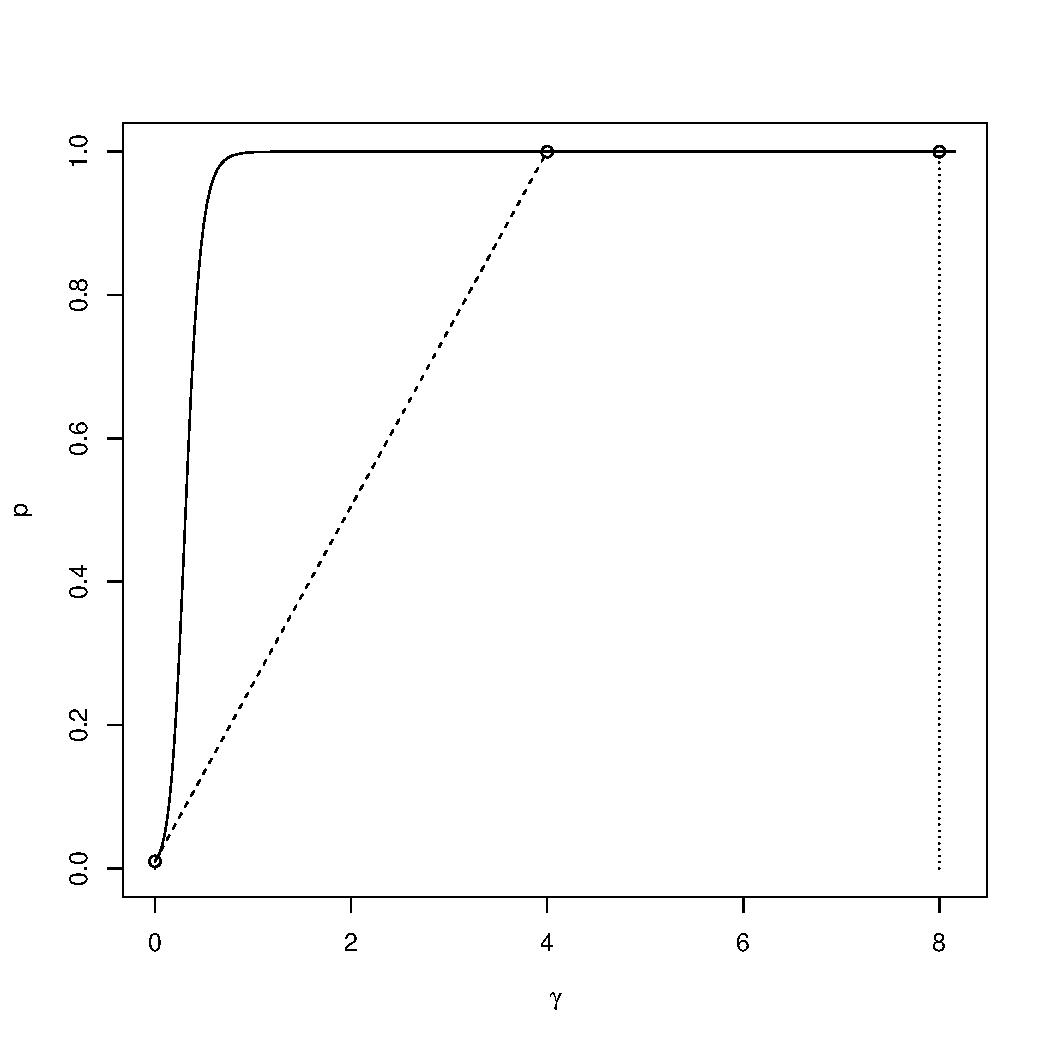
\includegraphics[width=3.35cm]{figs/trap1.pdf}}
\qquad
\subfloat[]{\label{fig:approx_5p} 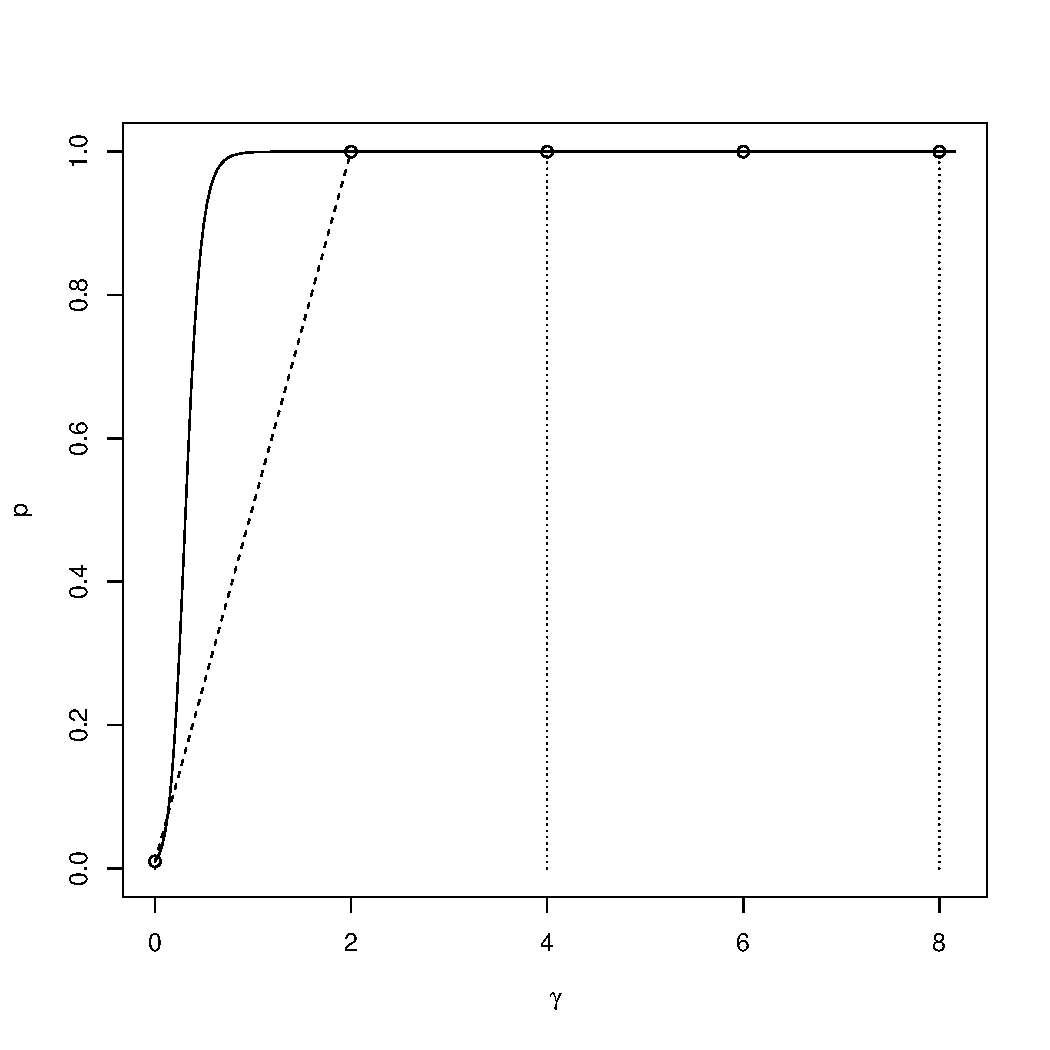
\includegraphics[width=3.35cm]{figs/trap2.pdf}}
\qquad
\subfloat[]{\label{fig:approx_7p} 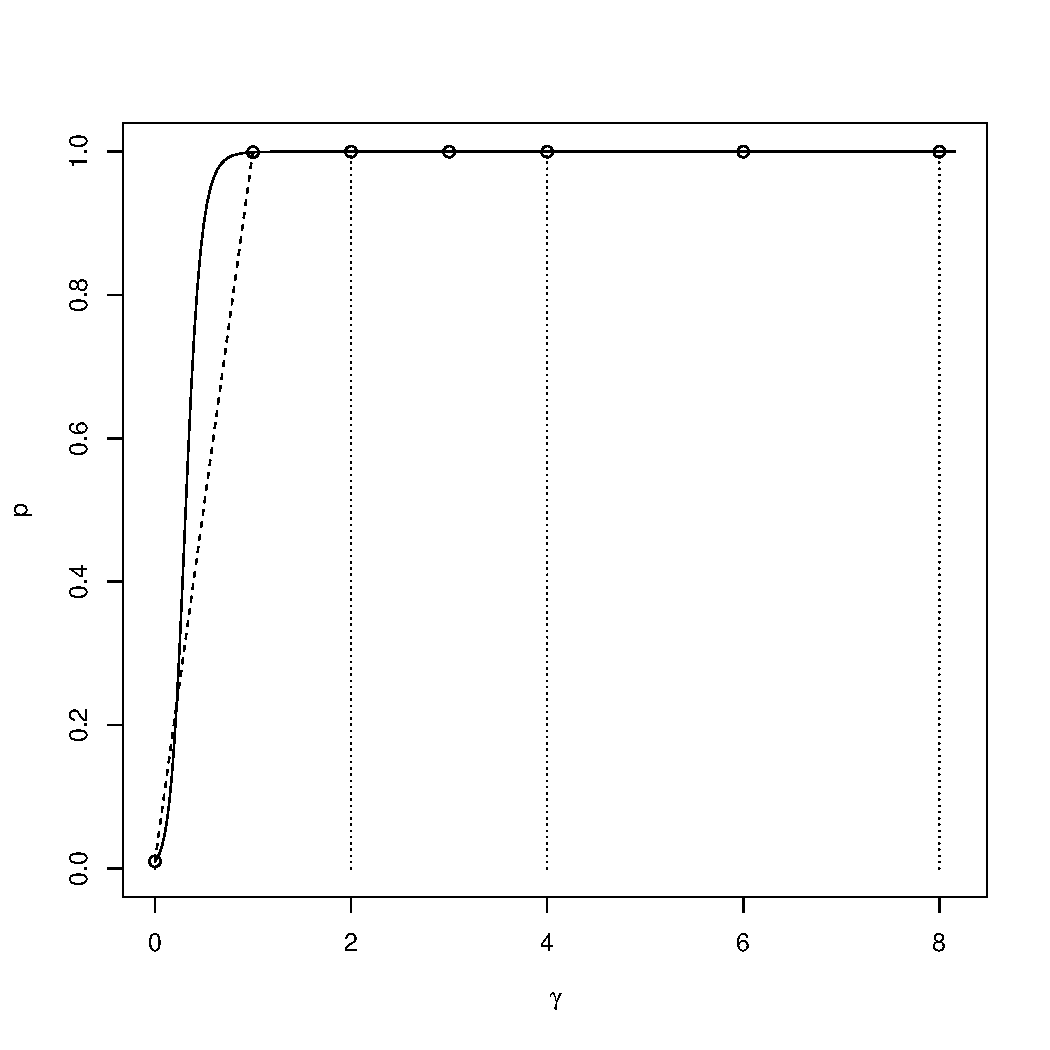
\includegraphics[width=3.35cm]{figs/trap3.pdf}}
\qquad
\subfloat[]{\label{fig:approx_21p} 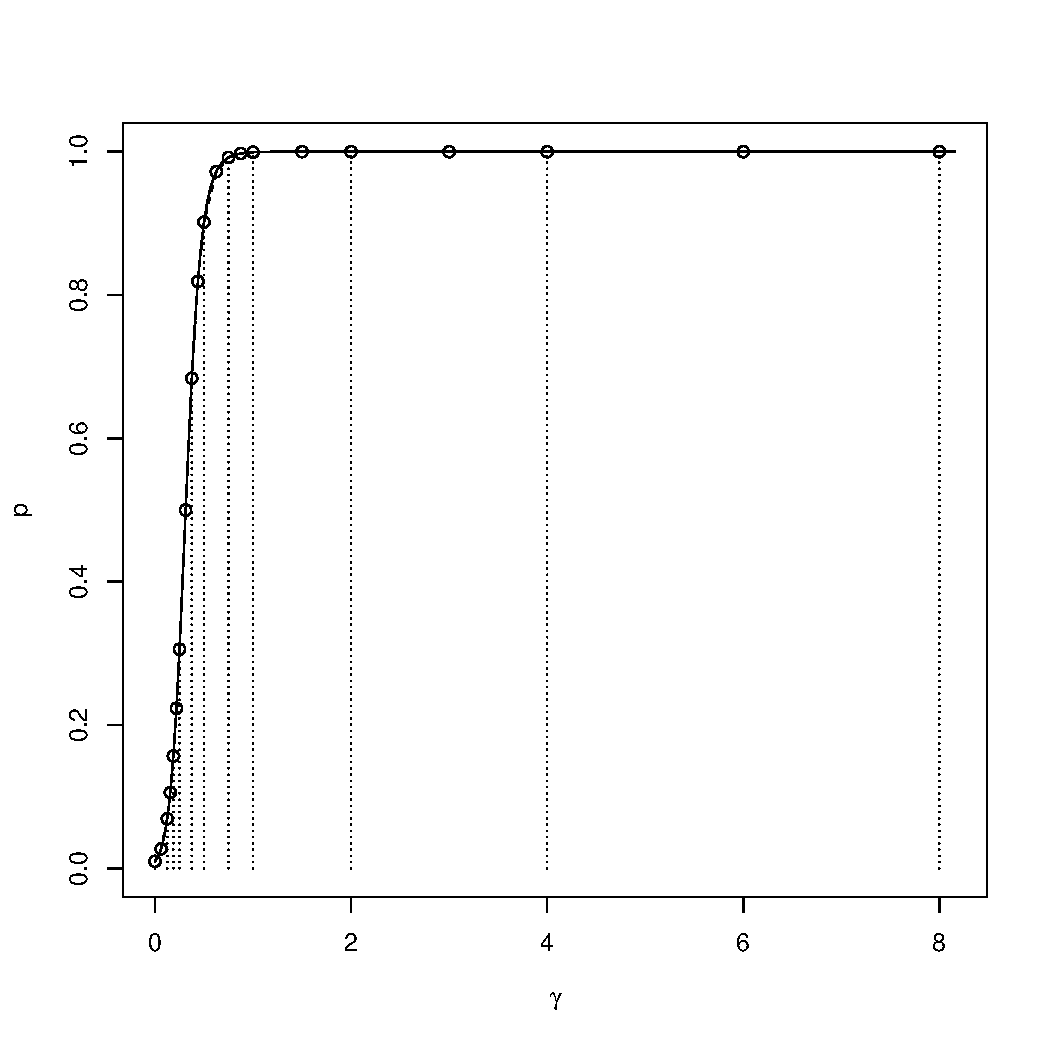
\includegraphics[width=3.35cm]{figs/trap6.pdf}}
\qquad
\subfloat[]{\label{fig:approx_3pcv2} 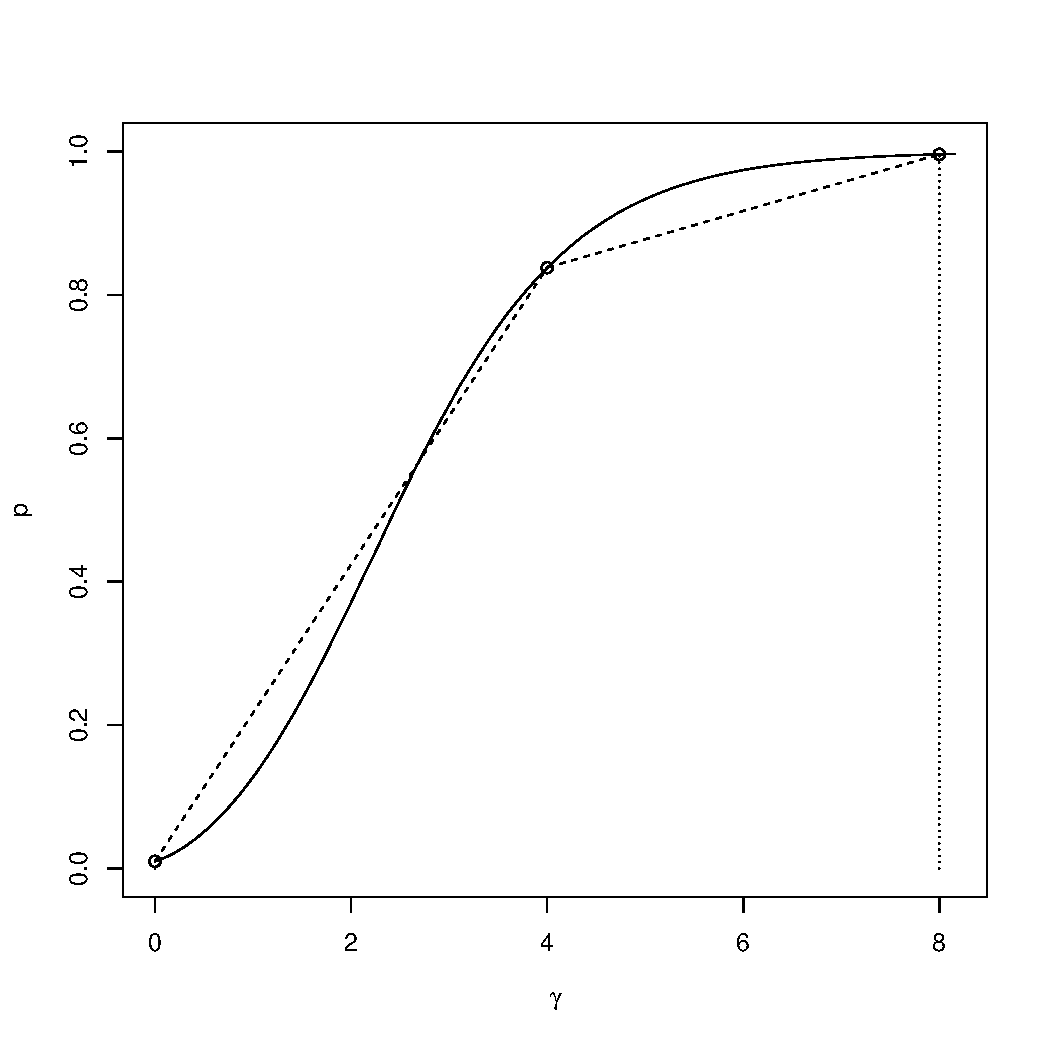
\includegraphics[width=3.35cm]{figs/trap21.pdf}}
\qquad
\subfloat[]{\label{fig:approx_5pcv2} 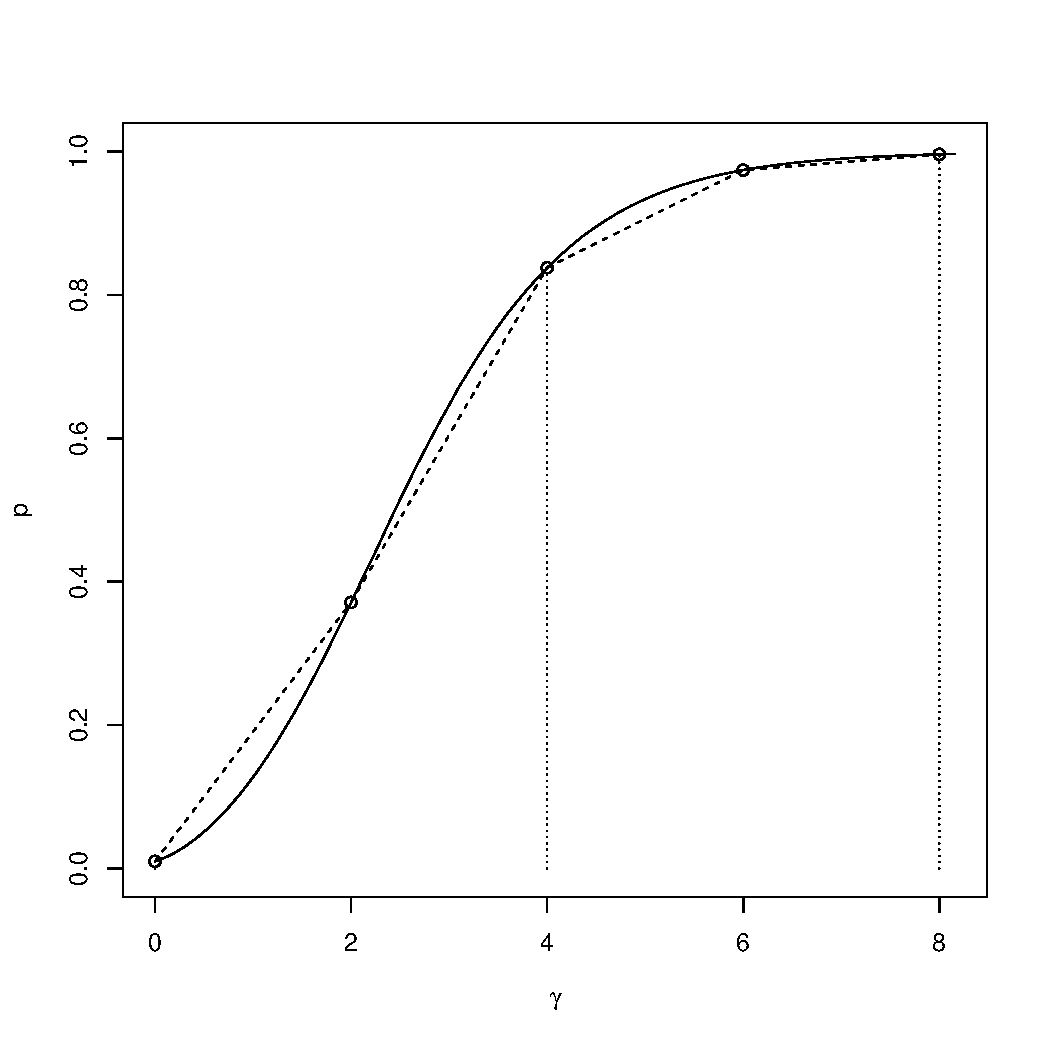
\includegraphics[width=3.35cm]{figs/trap22.pdf}}
\qquad
\subfloat[]{\label{fig:approx_9p} 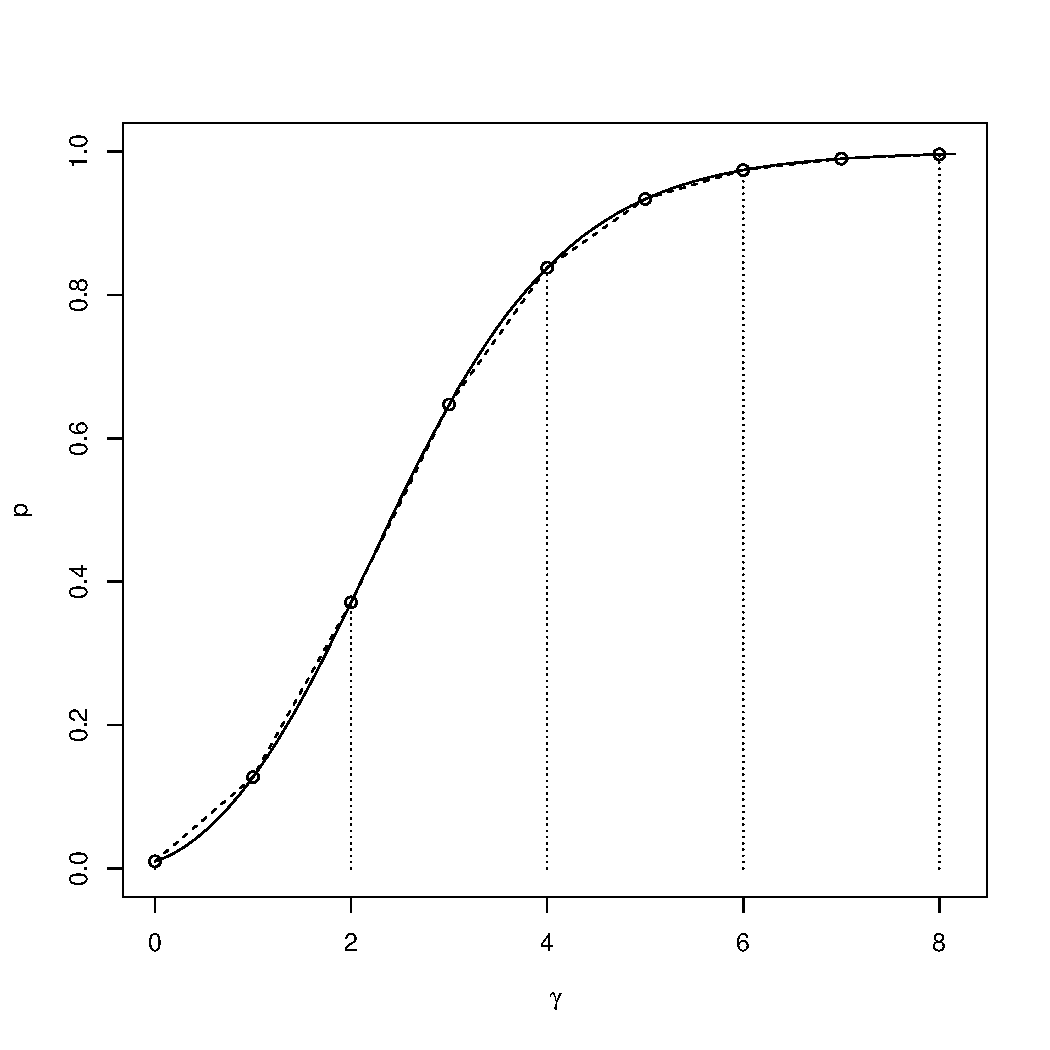
\includegraphics[width=3.35cm]{figs/trap23.pdf}}
\qquad
\subfloat[]{\label{fig:approx_3pcv3} 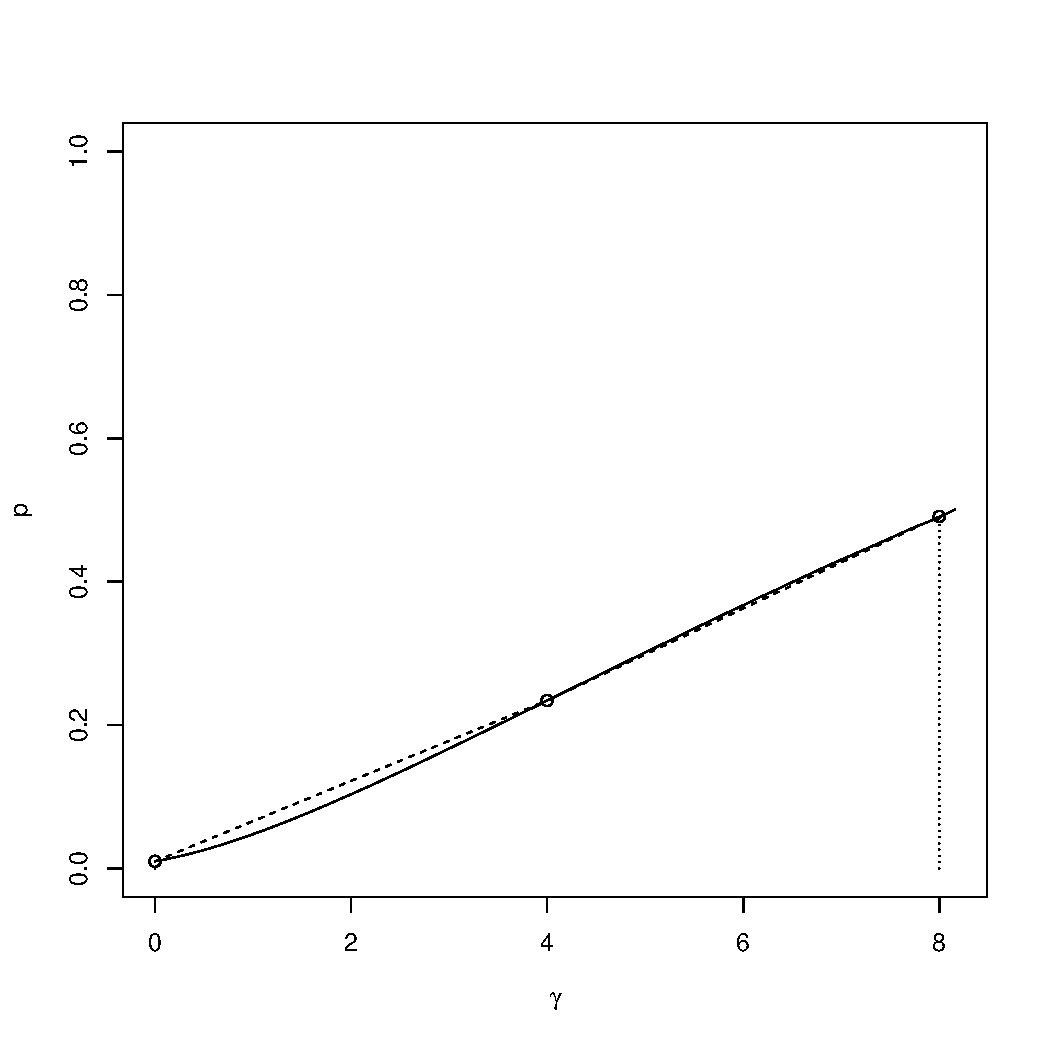
\includegraphics[width=3.35cm]{figs/trap31.pdf}}
\caption{}
\label{fig:approx_trap}
\end{figure}



\subsection{Observations' separability}

\subsection{Classifiers}
Whereas maximum margin classifiers are known for their high efficiency, they are also known for their high asymptotic computational complexity, due to this known high complexity, work in the literature has focused on the speeding up of these classifiers. Such work can be categorized into two approaches: \textit{algorithmic} and \textit{data-processing}. While the first approach devises algorithms to make the Quadratic Programming (QP) solver faster \cite{platt1998, keerthi2005}, the latter approach focuses on the selection of the training data, in order to reduce the number of training examples used ($N$) \cite{lee2001,panda2006}. Our approach to speeding up the computation of our index combines the best of both worlds, as well as we suggest the use of the fastest QP solver, we also elaborated an approach for selection of the training data.

The most straightforward approach to reduce $N$ is randomly down-sample the training dataset \cite{lee2001}. However, when evaluated the individual separability of an observation, it is necessary a more informed sampling, because the separability of the observation can be highly affected depending on the down-sampled observations. In Figure \ref{fig:knn_sampling} we can see two different sampling strategies from the dataset illustrated in the Figure \ref{fig:no_sampling} in order to evaluate the separability of the observation marked as red square. While the strategy adopted in the Figure \ref{fig:clump_sampling} completely modified the decision boundary due to the sampling of a single observation, the boundary of the Figure \ref{fig:cluster_sampling} remain the same, even with the sampling of a whole cluster.

\begin{figure}[h!]
\center
\subfloat[]{\label{fig:no_sampling} 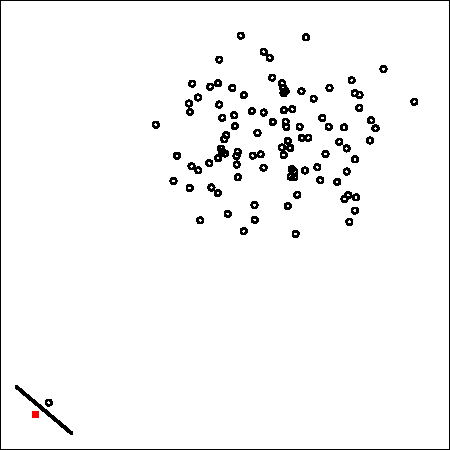
\includegraphics[width=4.7cm]{figs/knn1.pdf}}
\qquad
\subfloat[]{\label{fig:clump_sampling} 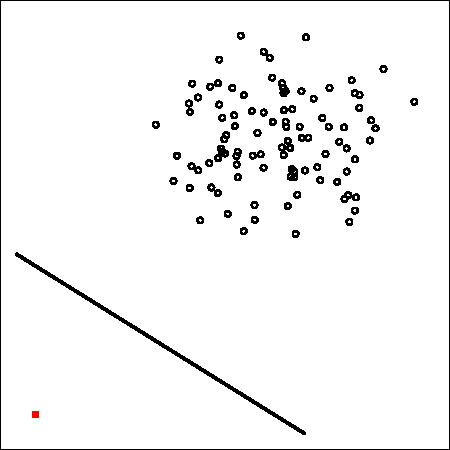
\includegraphics[width=4.7cm]{figs/knn2.pdf}}
\qquad
\subfloat[]{\label{fig:cluster_sampling} 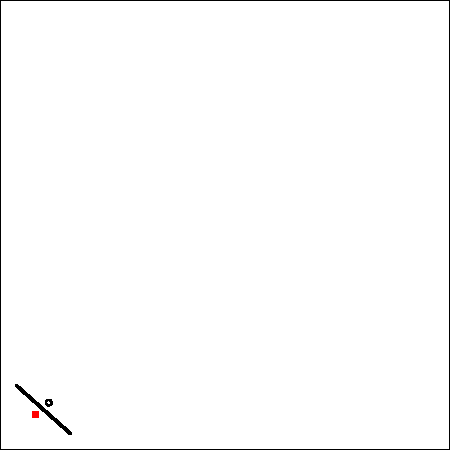
\includegraphics[width=4.7cm]{figs/knn3.pdf}}
\caption{}
\label{fig:knn_sampling}
\end{figure}

While the closest observations highly affected where the decision boundary will cut, the most distant observations are practically irrelevant, in fact, for certain classifiers, such as SVM, only the support vectors matters to make such decision. In order to select the most effective training subset, based on the work of \cite{panda2006}, we will use only the k-Nearest Neighbors (kNN) of the observation when its separability is evaluated. Note that in this problem, an approximate-NN approach \cite{gionis1999, schubert2015} is enough to select such observations.

Using this approach, the asymptotic computational complexity to compute the index for $s$ solutions goes from $\mathcal{O}(s \cdot n_{\gamma} \cdot N^4)$ to $\mathcal{O}(N^2 + s \cdot n_{\gamma} \cdot N \cdot k^3)$ when using a naive approach to compute the nearest neighbors, using the appropriate index structures, the computation can fall to $\mathcal{O}(N log N + s \cdot n_{\gamma} \cdot N \cdot k^3)$. In case of use the approximate-NN, the computation would cost $\mathcal{O}(N + s \cdot n_{\gamma} \cdot N \cdot k^3)$. It is important to note that most of the unsupervised outlier detection algorithms, which are the ones that benefit most from such internal indexes, also need to compute the nearest neighbors, this information can be reused for index computation and the complexity of the index would be only $\mathcal{O}(s \cdot n_{\gamma} \cdot N \cdot k^3)$.



=======
%\subsubsection{Adjustment for Chance}
%\subsubsection{Complexity}
%\subsubsection{Approximate Computation}
%\subsubsection{Internal Evaluation of Ranking Outlier Detection Results}
%scorings não dizem muito, simples ranking tera peso linear qndo não é recomendado pq dos inliers q sao maioria
%gammaMax
>>>>>>> parent of bf87337... merry xmas
\newpage